\chapter{Finanzierung}
\section{Zentrale Annahmen}
\begin{itemize}
	\item Förderungen/Zuschüsse sind nicht in den Berechnungen enthalten
	\item Keine Gewinnausschüttung bzw. Bonifikationen an die Unternehmensgründer
	\item Zahlungsziele (Kunden und Lieferanten): 30 Tage
\end{itemize}

\section{Finanzierungsmodell}
Die Finanzierung des Unternehmen erfolgt durch 4 Säulen. 

\noindent
\begin{tabular}{@{}>{\raggedright\arraybackslash}p{1.8cm}@{}>{\raggedright\arraybackslash}p{\textwidth - 1.8cm}}
 
	\textbf{Säule 1:} & Der Hersteller des Roboters finanziert die Anpassung des System an den jeweiligen Roboter mit der Entwicklungsgebühr. \\ 

	\textbf{Säule 2:} & Die Verwendung des Systems ist lizenziert. Für jeden Roboter, in dem das System zum Einsatz kommt, ist eine jährliche Lizenzgebühr fällig. Diese ist abhängig davon, wie viel Einsparungspotential durch das System möglich ist und welche Version des Systems verwendet wird. \\
	
	\textbf{Säule 3:} & Der Roboterhersteller finanziert eine Weiterentwicklung eines bestehenden Systems. \\
	
	\textbf{Säule 4:} & Damit der Betreiber das System verwenden müssen seine Mitarbeiter geschult werden.
\end{tabular}

\subsection{Entwicklungsgebühr}
\subsubsection{Neuentwicklung}
Die Entwicklungsgebühr ist unabhängig vom Roboter und Hersteller. Sie stützt sich darauf, dass der Roboter für die Betreiber attraktiver wird, da dieser eine jährliche Stromersparnis und dadurch resultierende Kostenersparnis mit sich bringt.\\
Die Entwicklungsgebühr beträgt $100.000,00$\officialeuro.\\
Diese kann um bis zu $20$\% verringert werden sofern entsprechende Gegenleistungen angeboten werden.

\subsubsection{Weiterentwicklung}
Das grundlegende System unterliegt einer ständigen Weiterentwicklung. Neue Versionen des System müssen jedoch wieder an einen Roboter angepasst werden. Abhängig von den Versionsunterschieden beträgt die Gebühr zwischen $25.000$ und $50.000$\officialeuro.\\
Diese kann um bis zu $20$\% verringert werden sofern entsprechende Gegenleistungen angeboten werden.

\subsection{Lizenzgebühren}
Die Verwendung des Systems verschafft dem Betreiber einen enormen Wettbewerbsvorteil. Damit der Betreiber das System verwenden kann ist eine zurzeit eine einmalige Lizenzgebühr pro Roboter fällig. Sie wird wie folgt berechnet:\\
\begin{align*}
	Gebühr = (((24h * 365d * \varnothing A)*P_N)*\varnothing K_{Strom}*E_N)*\frac{\varnothing B_N}{2} + IBN
\end{align*}
\begin{tabbing}
	\hspace{1,8cm}\=\hspace{0,6cm}\=\kill
	$\varnothing A$ \> \dots \> durchschnittliche Auslastung des Roboters in einem Jahr $[\%]$\\ 
	$P_N$\> \dots \> nominelle Leistungsaufnahme des Roboters bei deaktiviertem System\\ 
	\> \> (wird durch den eigenen Messaufbau festgelegt)\\
	$\varnothing K_{Strom}$\> \dots \> durchschnittliche gewerbliche Stromkosten\\ 
	$E_N$\> \dots \> Effizientssteigerung durch das System\\ 
	\> \> (wird durch den eigenen Messaufbau festgelegt) \\
	$\varnothing B_N$ \> \dots \> durchschnittliche nominelle Betriebsdauer des Roboters \\
	$IBN$ \> \dots \> Pauschale zur Inbetriebnahme
\end{tabbing}
Die Werte $P_N$ und $E_N$ sind abhängig von der Version des Systems und werden für diese immer neu ermittelt. Die durchschnittliche Betriebsdauer $\varnothing B_N$ wird mit $10$ Jahren festgelegt und die durchschnittliche Auslastung $\varnothing A$ mit $70$\%. Ausnahmen können mit dem Betreiber explizit verhandelt werden. Die $IBN$-Pauschaule ist ebenfalls ein Fixwert und mit $350$\officialeuro festgelegt. Für die durchschnittlichen Stromkosten wird der offizielle Wert der \textsf{E-CONTROL}\footnote{Energie-Control Austria für die Regulierung der Elektrizitäts- und Erdgaswirtschaft, Rudolfsplatz 13a, 1010 Wien} für Nicht-Haushalte und über $150.000$MWh/a herangezogen.\\
Für die \textit{Version 1} des Systems ergeben sich somit die Werte in Tabelle \ref{tab:Kalkulationswerte}.
\begin{table}[h]
\centering
\begin{tabular}{|c|c|}
	\hline 
	$\varnothing A$ & $70$\% \\ 
	\hline 
	$\varnothing K_{Strom}$ & $5,418\frac{\text{Cent}}{\text{kWh}}$ \\ 
	\hline
	$\varnothing B_N$ & $10$ Jahre \\ 
	\hline 
	$IBN$ & $350$\officialeuro \\ 
	\hline 
\end{tabular}
\caption{Kalkulationswerte für \textit{Version 1}}
\label{tab:Kalkulationswerte}
\end{table}
Eine grafische Verteilung der Lizenzgebühren für $E_N = 5,00$\% -- $50,00$\% und $P_N = 0,5$kW -- $10,0$kW ist in Abbildung \ref{fig:lizenzgebuehr} dargestellt.

\begin{figure}[h]
	\centering
	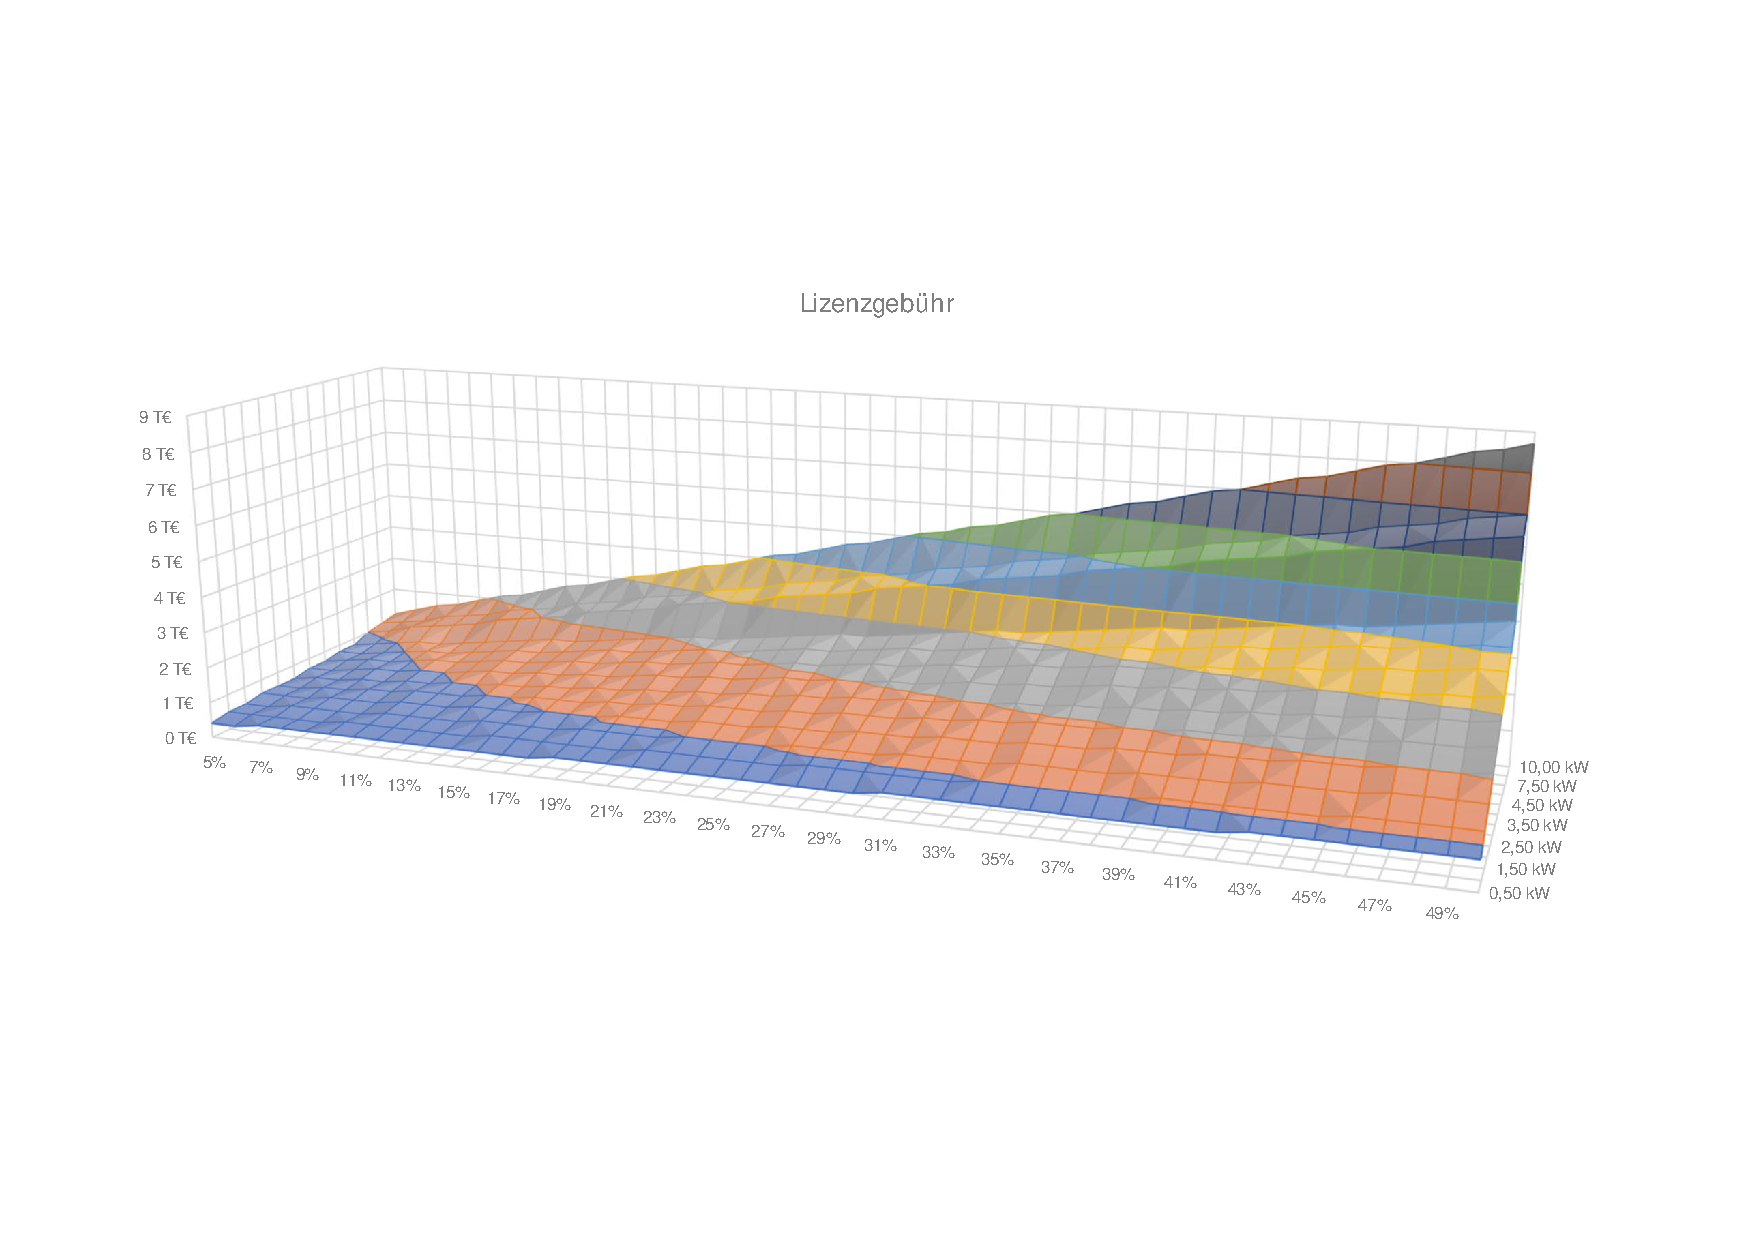
\includegraphics[width=15cm]{Lizenzgebuehr.pdf}
	\caption{Lizenzgebühr für die \textit{Version 1}}
	\label{fig:lizenzgebuehr}
\end{figure}

\paragraph*{Versionsupdate:}
Wird eine neue Version veröffentlicht, ist es für jeden Betreiber möglich auf das neue System upzudaten. Damit wird aber auch die Lizenzgebühr entsprechend angepasst. Außerdem wird die entsprechende $IBN$-Pauschale verrechnet.

\subsection{Schulung}
\subsubsection{Grundschulung}
Die Grundschulung umfasst die Installation und Verwendung des System mit der Robotersteuerung. Die Schulung dauert 2 Tage und die Kosten betragen $800,00$\officialeuro~pro Person.

\subsubsection{Intensivschulung}
Im System können Parameter verändert werden um mögliche spezielle Anforderungen abdecken zu können. Wie die Parameter verändert werden können und welche Auswirkung die Veränderungen haben ist Teil der Intensivschulung. Diese dauert 3 Tage und die Kosten betragen $1.500,00$\officialeuro~pro Person.

\section{Basis-Scenario}
Für das Basis-Scenario wurden folgende Annahmen getroffen:
\begin{itemize}
	\item Es werden in den folgenden 4 Jahren 20 Neuentwicklungen in Auftrag gegeben (Aufteilung:~3/5/6/6). Damit werden $~12$\% der Robotertypen der 5 wichtigsten Hersteller mit dem System ausgerüstet, siehe Kapitel \ref{sec:Marketing}.
	\item Die Lizenzvergabe verteilt sich wie folgt:\newline (Angaben in Prozent vom weltweitem Absatz von Industrierobotern ($400.000$ Stück), siehe Kapitel \ref{sec:Marketing})
	\begin{itemize}
		\item 1. Jahr: $0,00$\% (0 Roboter)
		\item 2. Jahr: $0,03$\% (~120 Roboter)
		\item 3. Jahr: $0,09$\% (~360 Roboter)
		\item 4. Jahr: $0,25$\% (~1000 Roboter)
	\end{itemize}
	\item Die durchschnittliche Lizenzgebühr beträgt $1.500,00$\officialeuro.\\ Dies entspricht dem Mittelwert für $P_N = 1,50$kW -- $5,00$kW und $E_N = 10$\% -- $30$\%.
	\item Es wird mit 60 Teilnehmer an der Grundschulung innerhalb der nächsten 4 Jahren gerechnet (Aufteilung:~8/12/16/24). Zusätzlich nehmen 10 Teilnehmer die Intensivschulung in Anspruch (Aufteilung: 0/2/3/5).
\end{itemize}

\subsection{Break-Even-Point}
Der BEP wird im Basis-Szenario im 3. Jahr erreicht, siehe Abbildung \ref{fig:BasisSzenario-BEP}.
\begin{figure}[h]
	\centering
	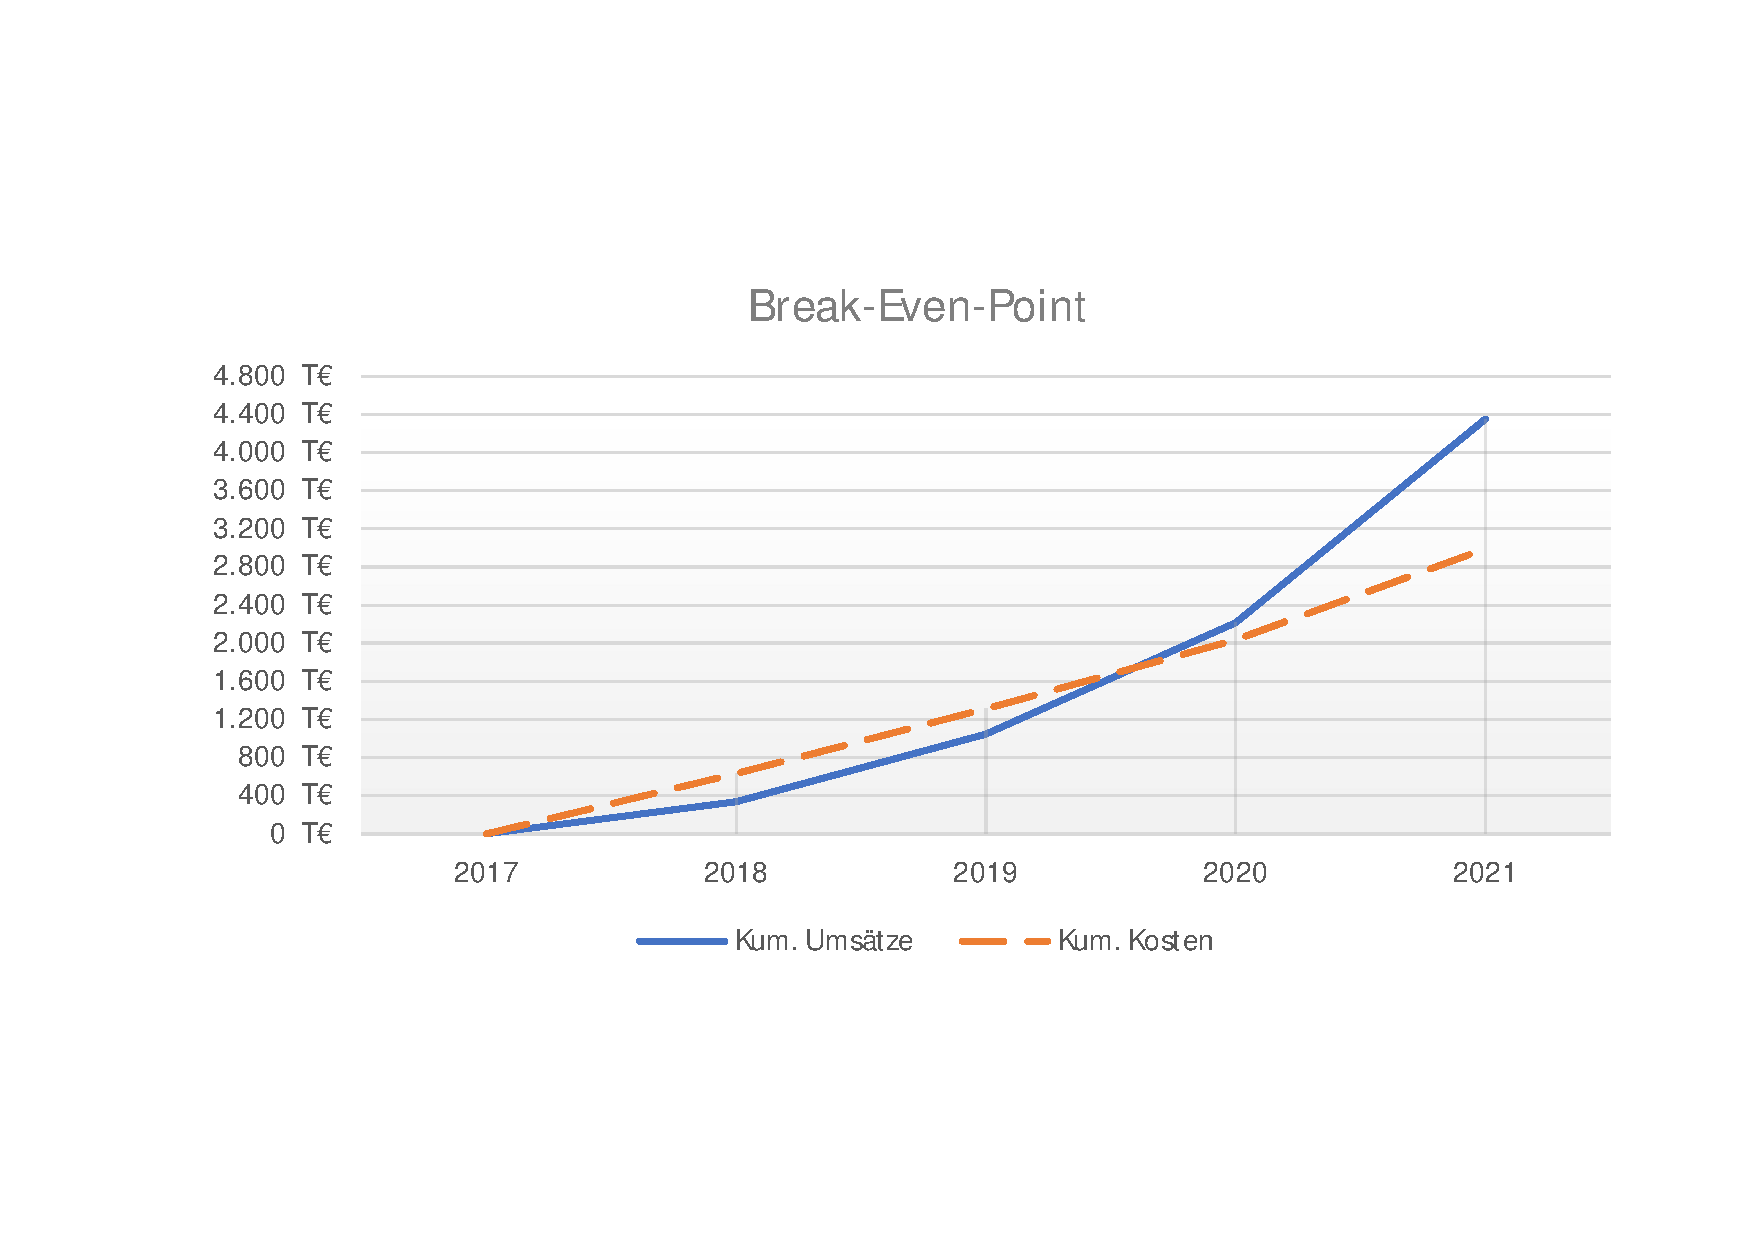
\includegraphics[width=15cm]{BasisSzenario-BEP.pdf}
	\caption{Break-Even-Point im Basis-Szenario}
	\label{fig:BasisSzenario-BEP}
\end{figure}

\subsection{Kapitalbedarf}
Der Kapitalbedarf bis zum BEP beträgt höchstens $220.000$\officialeuro.\\
Um diese Lücke zu schließen, werden folgende Finanzierungsmöglichkeiten geplant:
\begin{itemize}
	\item Einreichung eines Antrags bei der FFG im Basisprogramm zur Förderung von Einzelprojekten.
	\item UBG Gründerfonds
	\item Zusätzliches Eigenkapital
\end{itemize}
Dadurch ergibt sich folgende Finanzierung:\\
\begin{tabular}{l r}
	Kapitalbedarf & $-220.000$\officialeuro \\
	\hline
	FFG Basisprogramm(Projektsumme: $200.000$\officialeuro) & $+100.000$\officialeuro \\
	UBG Gründerfond & $+75.000$\officialeuro \\
	Zusätzliches Eigenkapital & $+45.000$\officialeuro \\
	\bottomrule
\end{tabular}\\

\noindent Kurzfristige Liquiditätsschwankungen (spätere Zahlungen der Kunden, Projektvorfinanzierung, …) werden mit einem Kontokorrentkredit abgedeckt.

\subsection{Kennzahlen}
\begin{figure}[h]
	\centering
	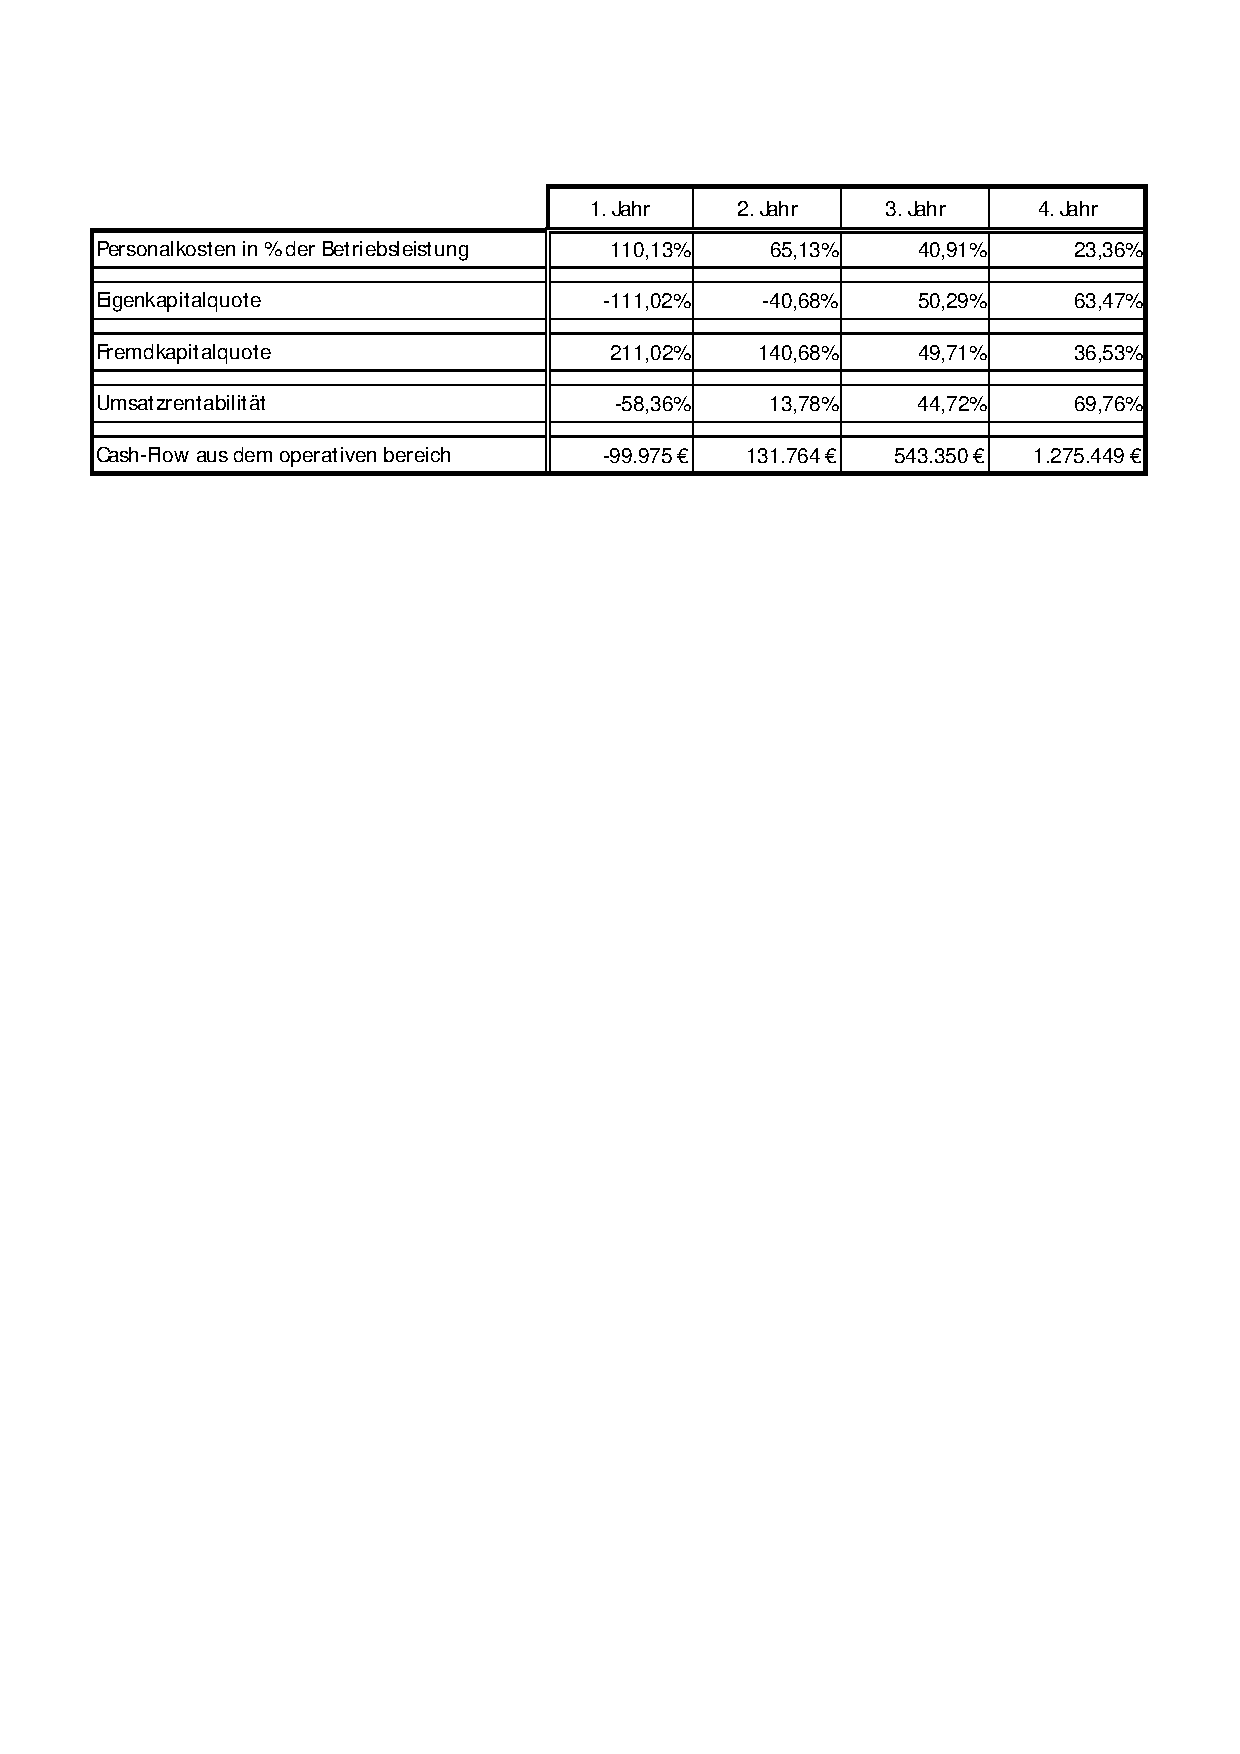
\includegraphics[width=15cm]{BasisSzenario-Kennzahlen.pdf}
	\caption{Kennzahlen im Basis-Szenario}
	\label{fig:BasisSzenario-Kennzahlen}
\end{figure}
\newpage
\subsection{Planbilanz}
\begin{figure}[h]
	\centering
	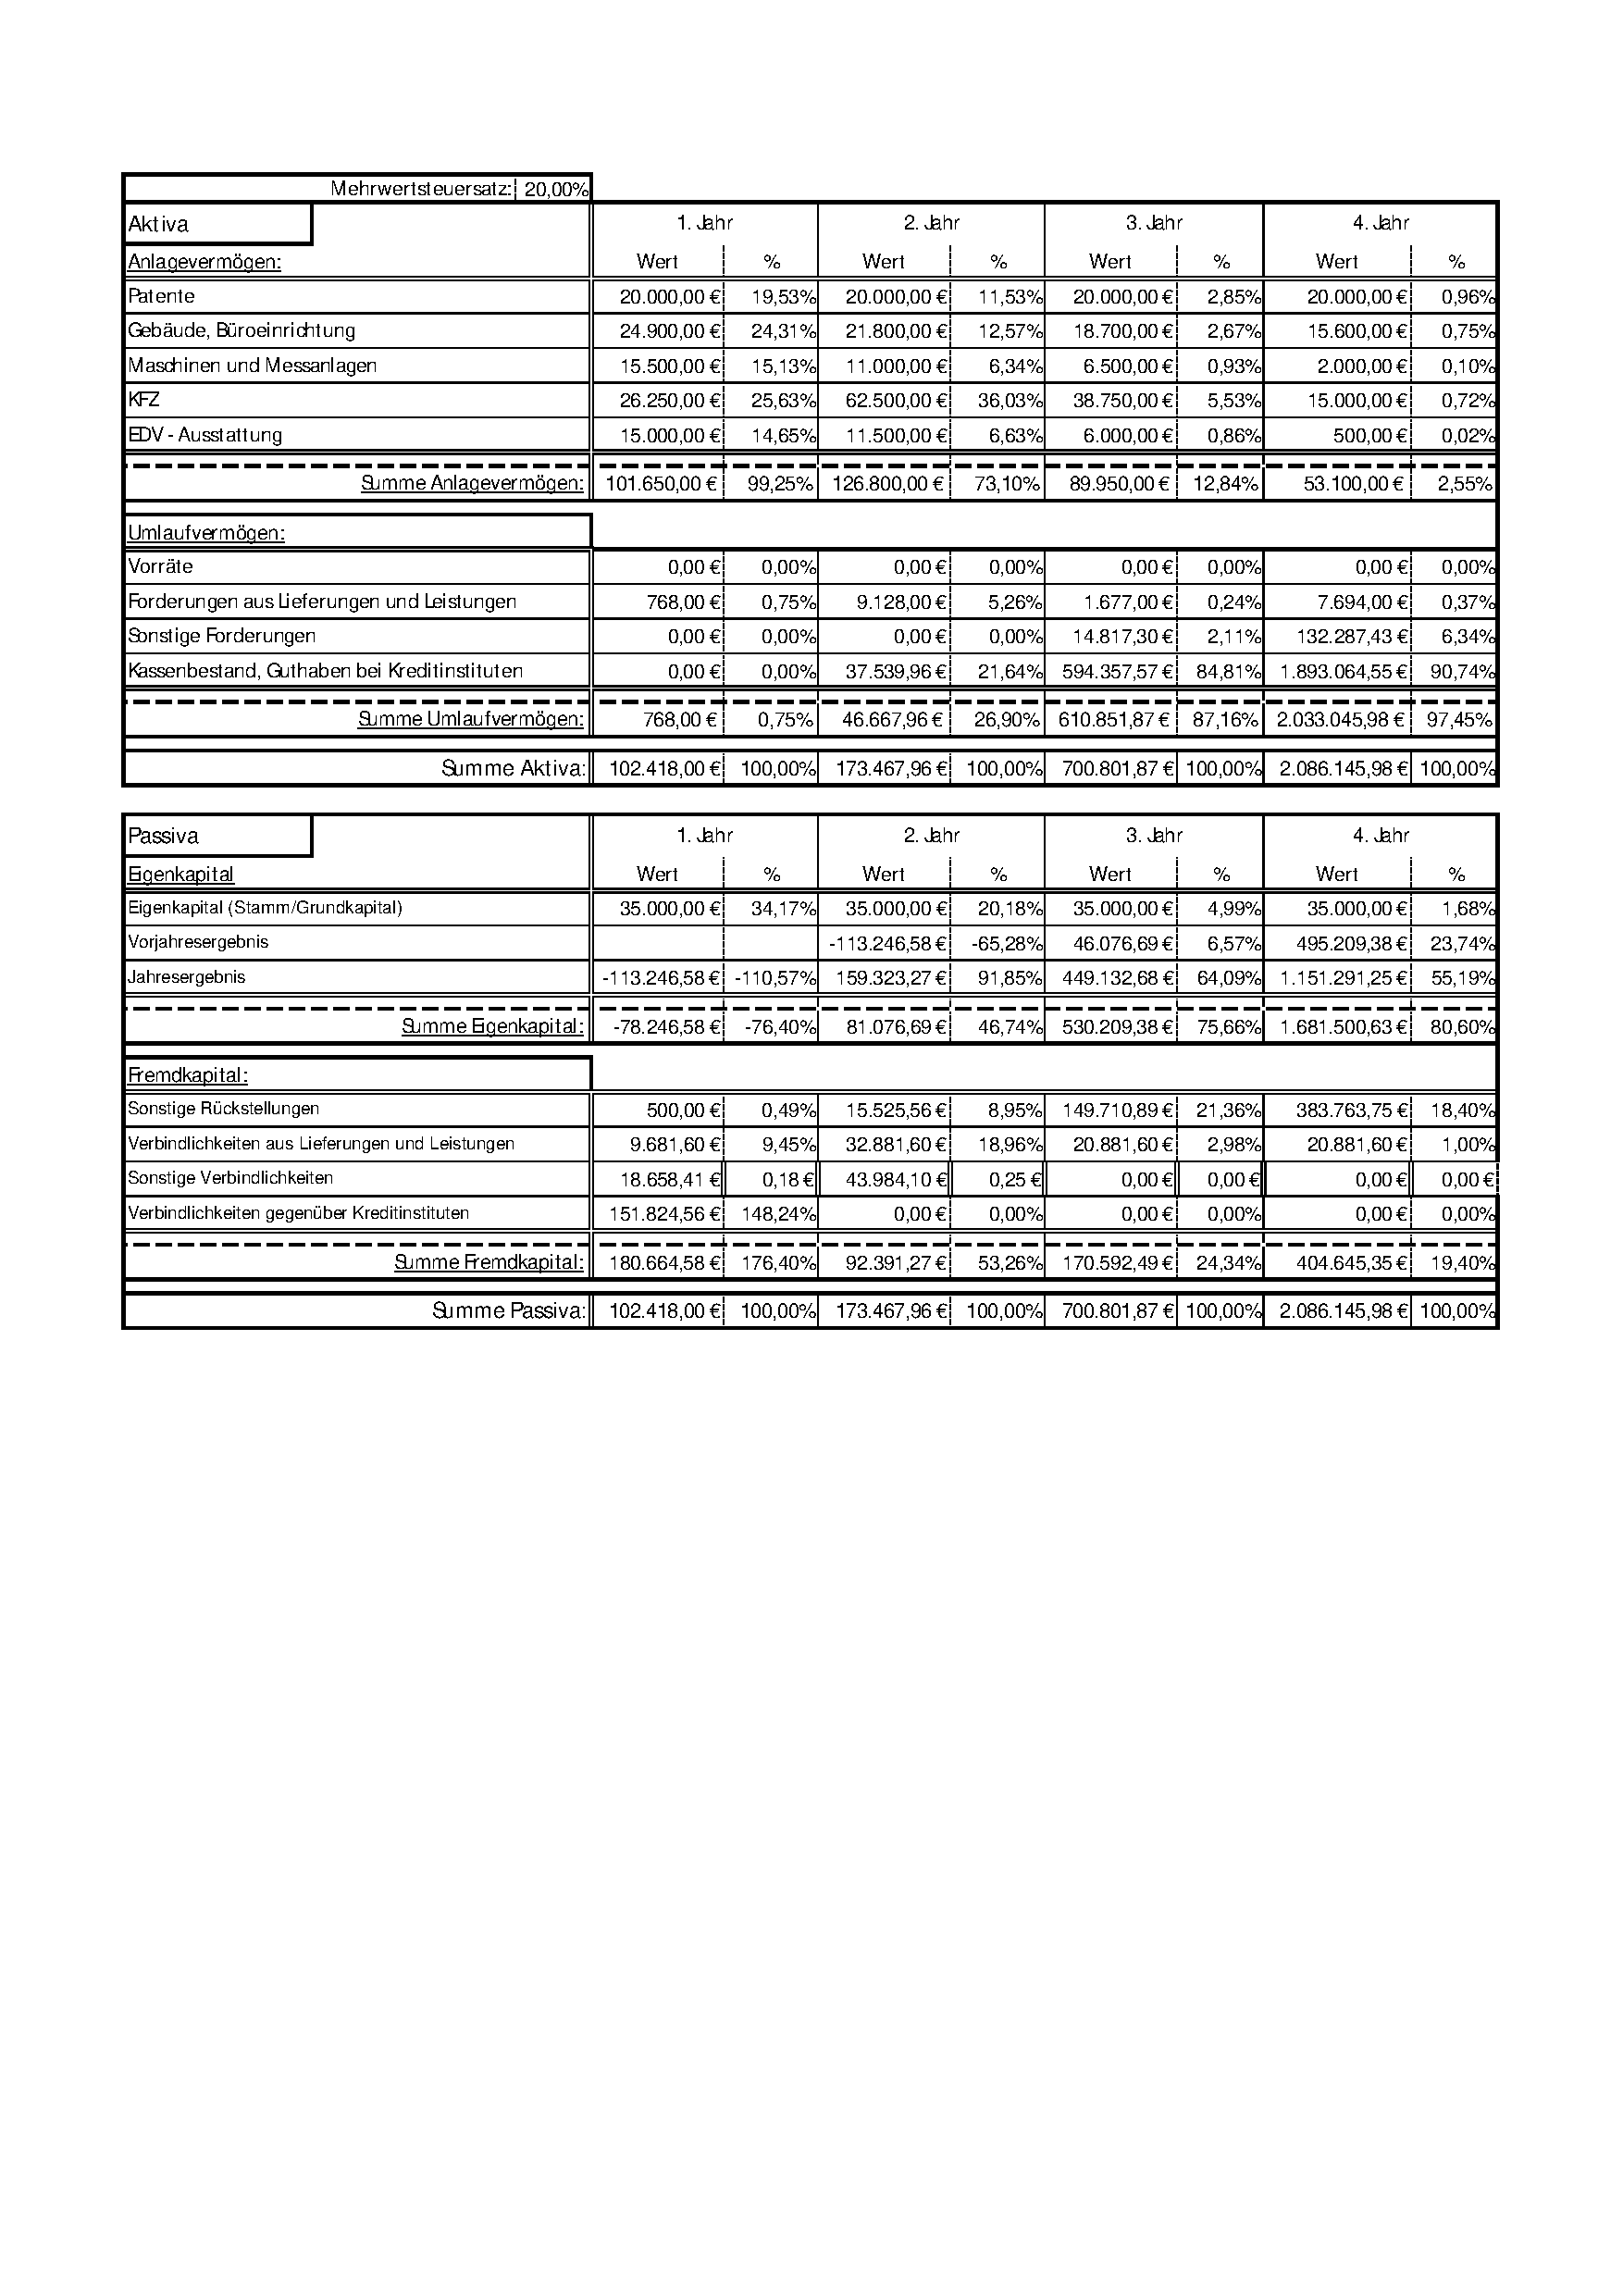
\includegraphics[width=15cm]{BasisSzenario-Planbilanz.pdf}
	\caption{Planbilanz im Basis-Szenario}
	\label{fig:BasisSzenario-Planbilanz}
\end{figure}

\newpage
\subsection{Liquiditätsplan}
\begin{figure}[htp!]
	\centering
	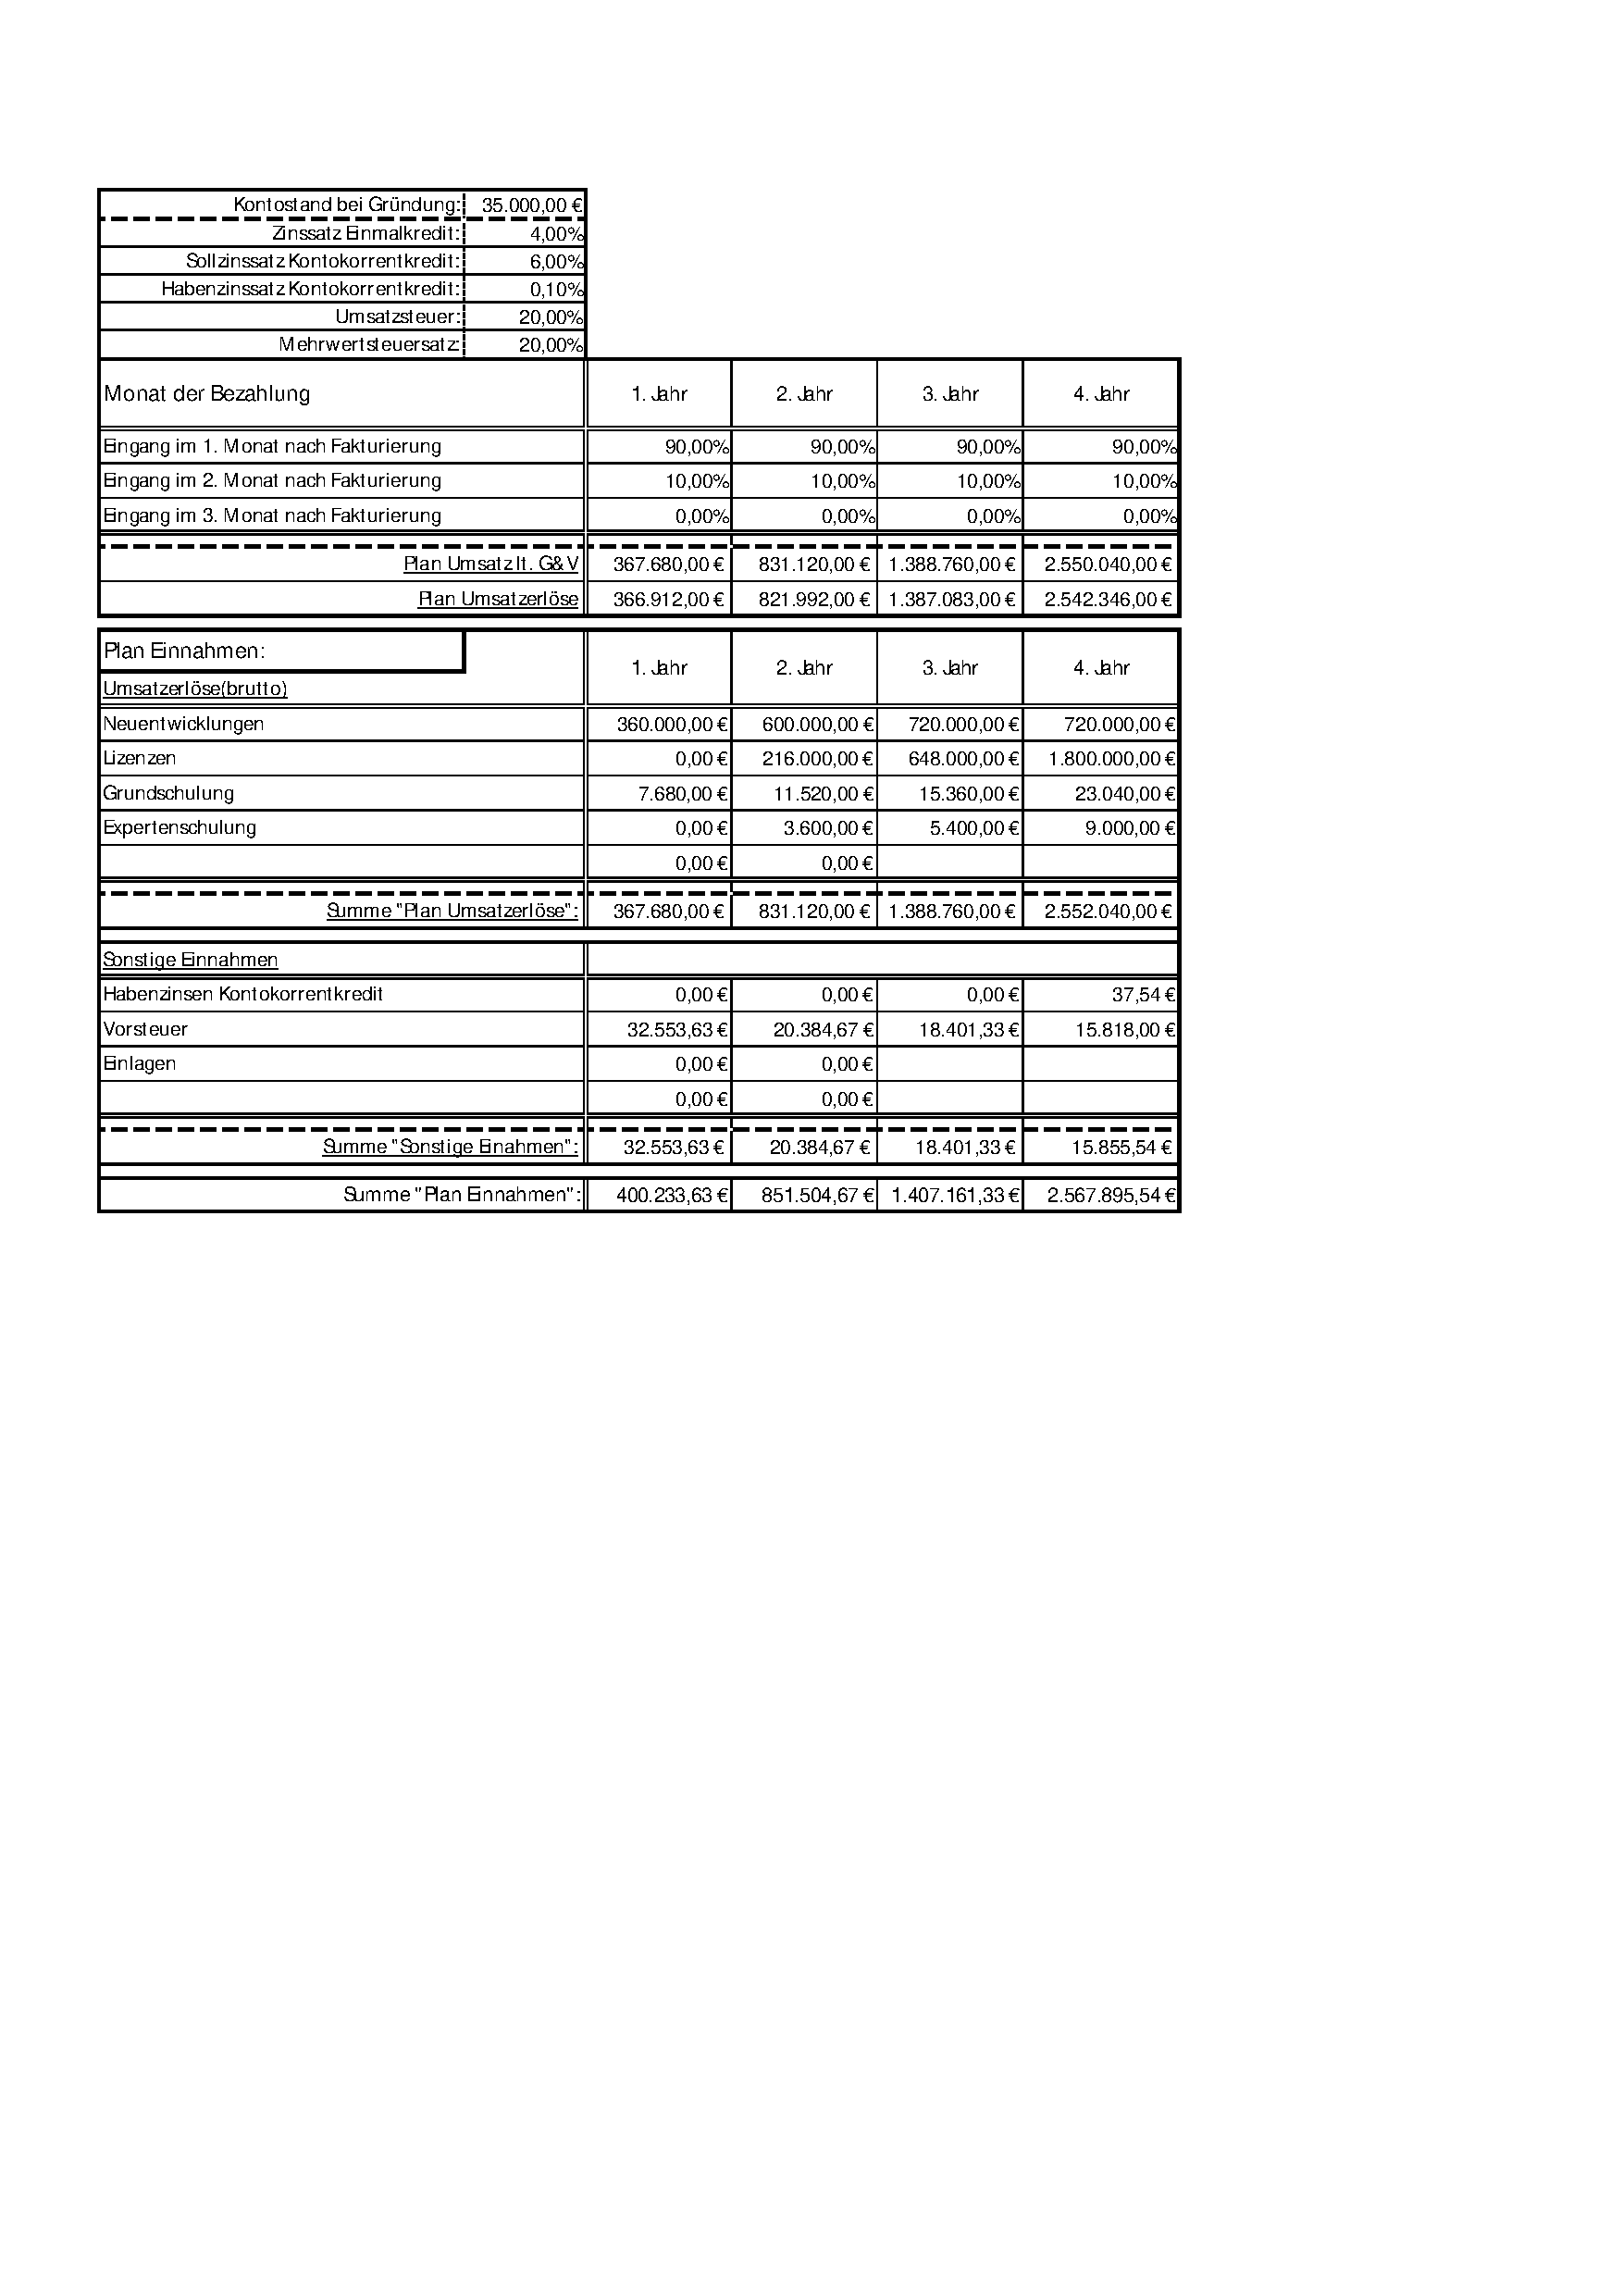
\includegraphics[page=1,width=15cm]{BasisSzenario-Liquiditaet.pdf}
	\label{fig:BasisSzenario-Liquiditaet-1}
\end{figure}
\begin{figure}[htp!]
	\centering
	\includegraphics[page=2,width=15cm]{BasisSzenario-Liquiditaet.pdf}
	\caption{Liquiditätsplan im Basis-Szenario}
	\label{fig:BasisSzenario-Liquiditaet-2}
\end{figure}

\newpage
\subsection{Plan Gewinn- \& Verlustrechnung}
\begin{figure}[htp!]
	\centering
	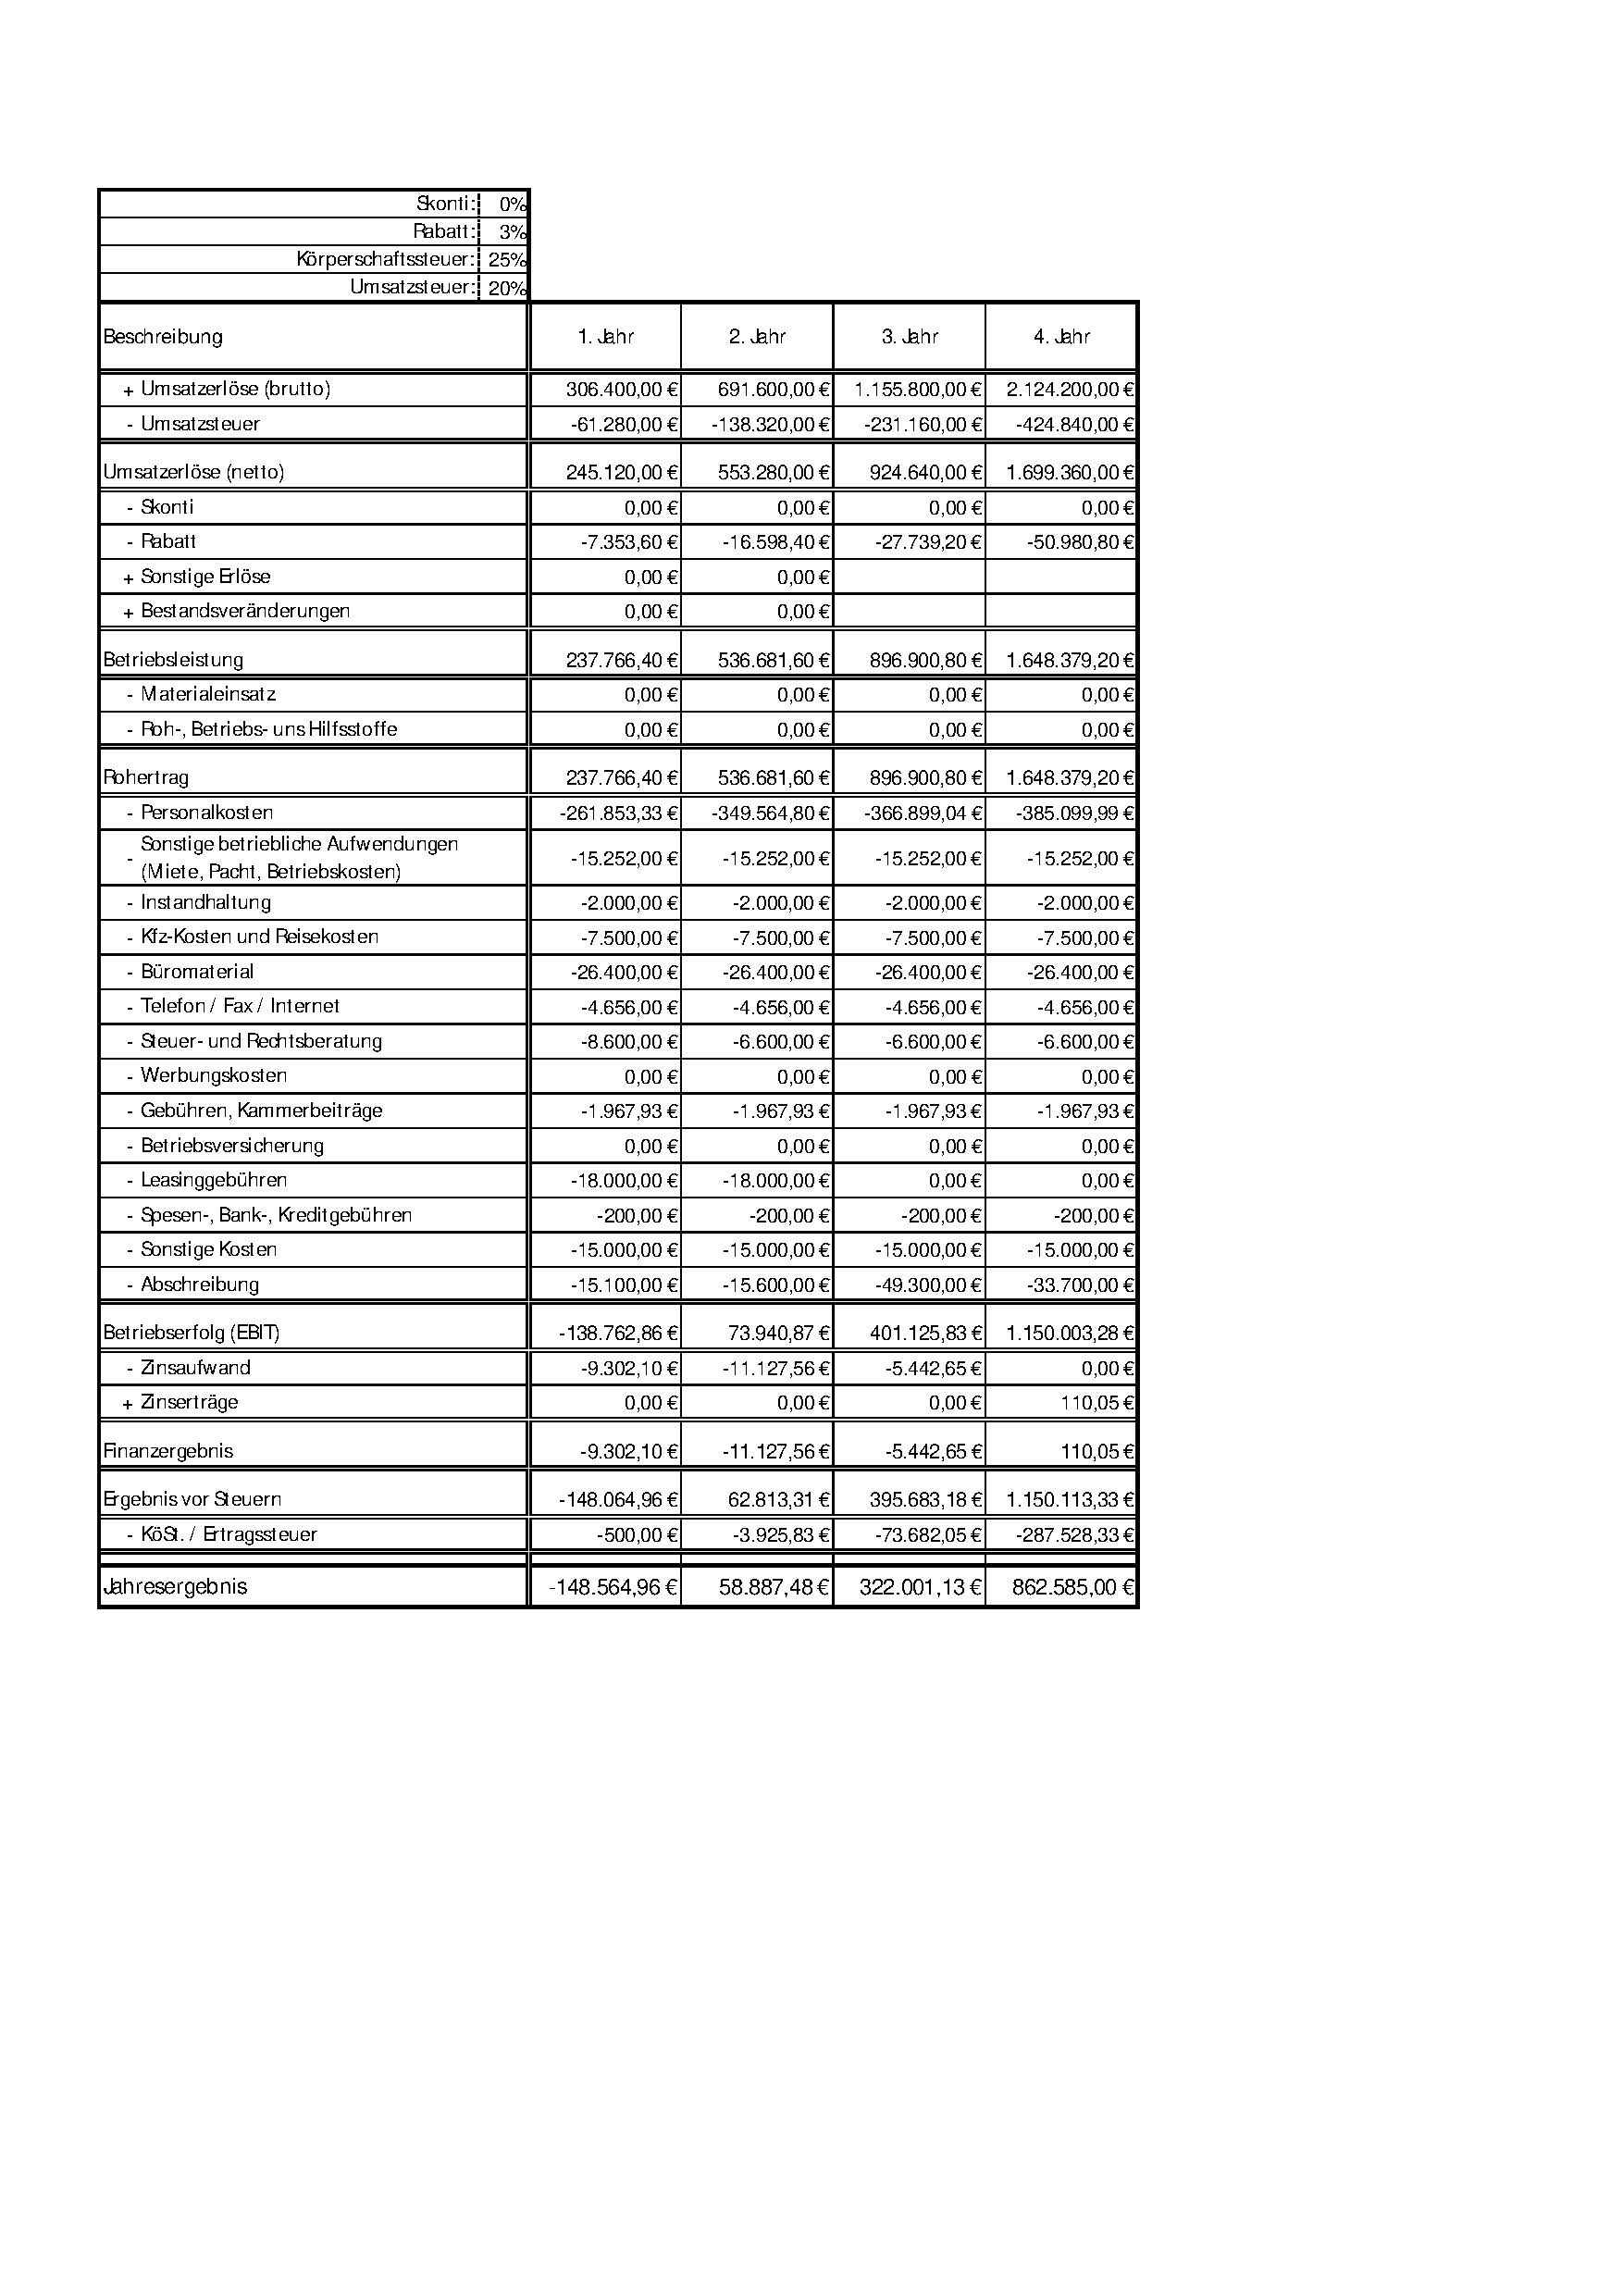
\includegraphics[width=15cm]{BasisSzenario-PlanGuV.pdf}
	\caption{Gewinn- \& Verlustrechnung im Basis-Szenario}
	\label{fig:BasisSzenario-GuV}
\end{figure}

\newpage
\subsection{Investition}
\begin{figure}[htp!]
	\centering
	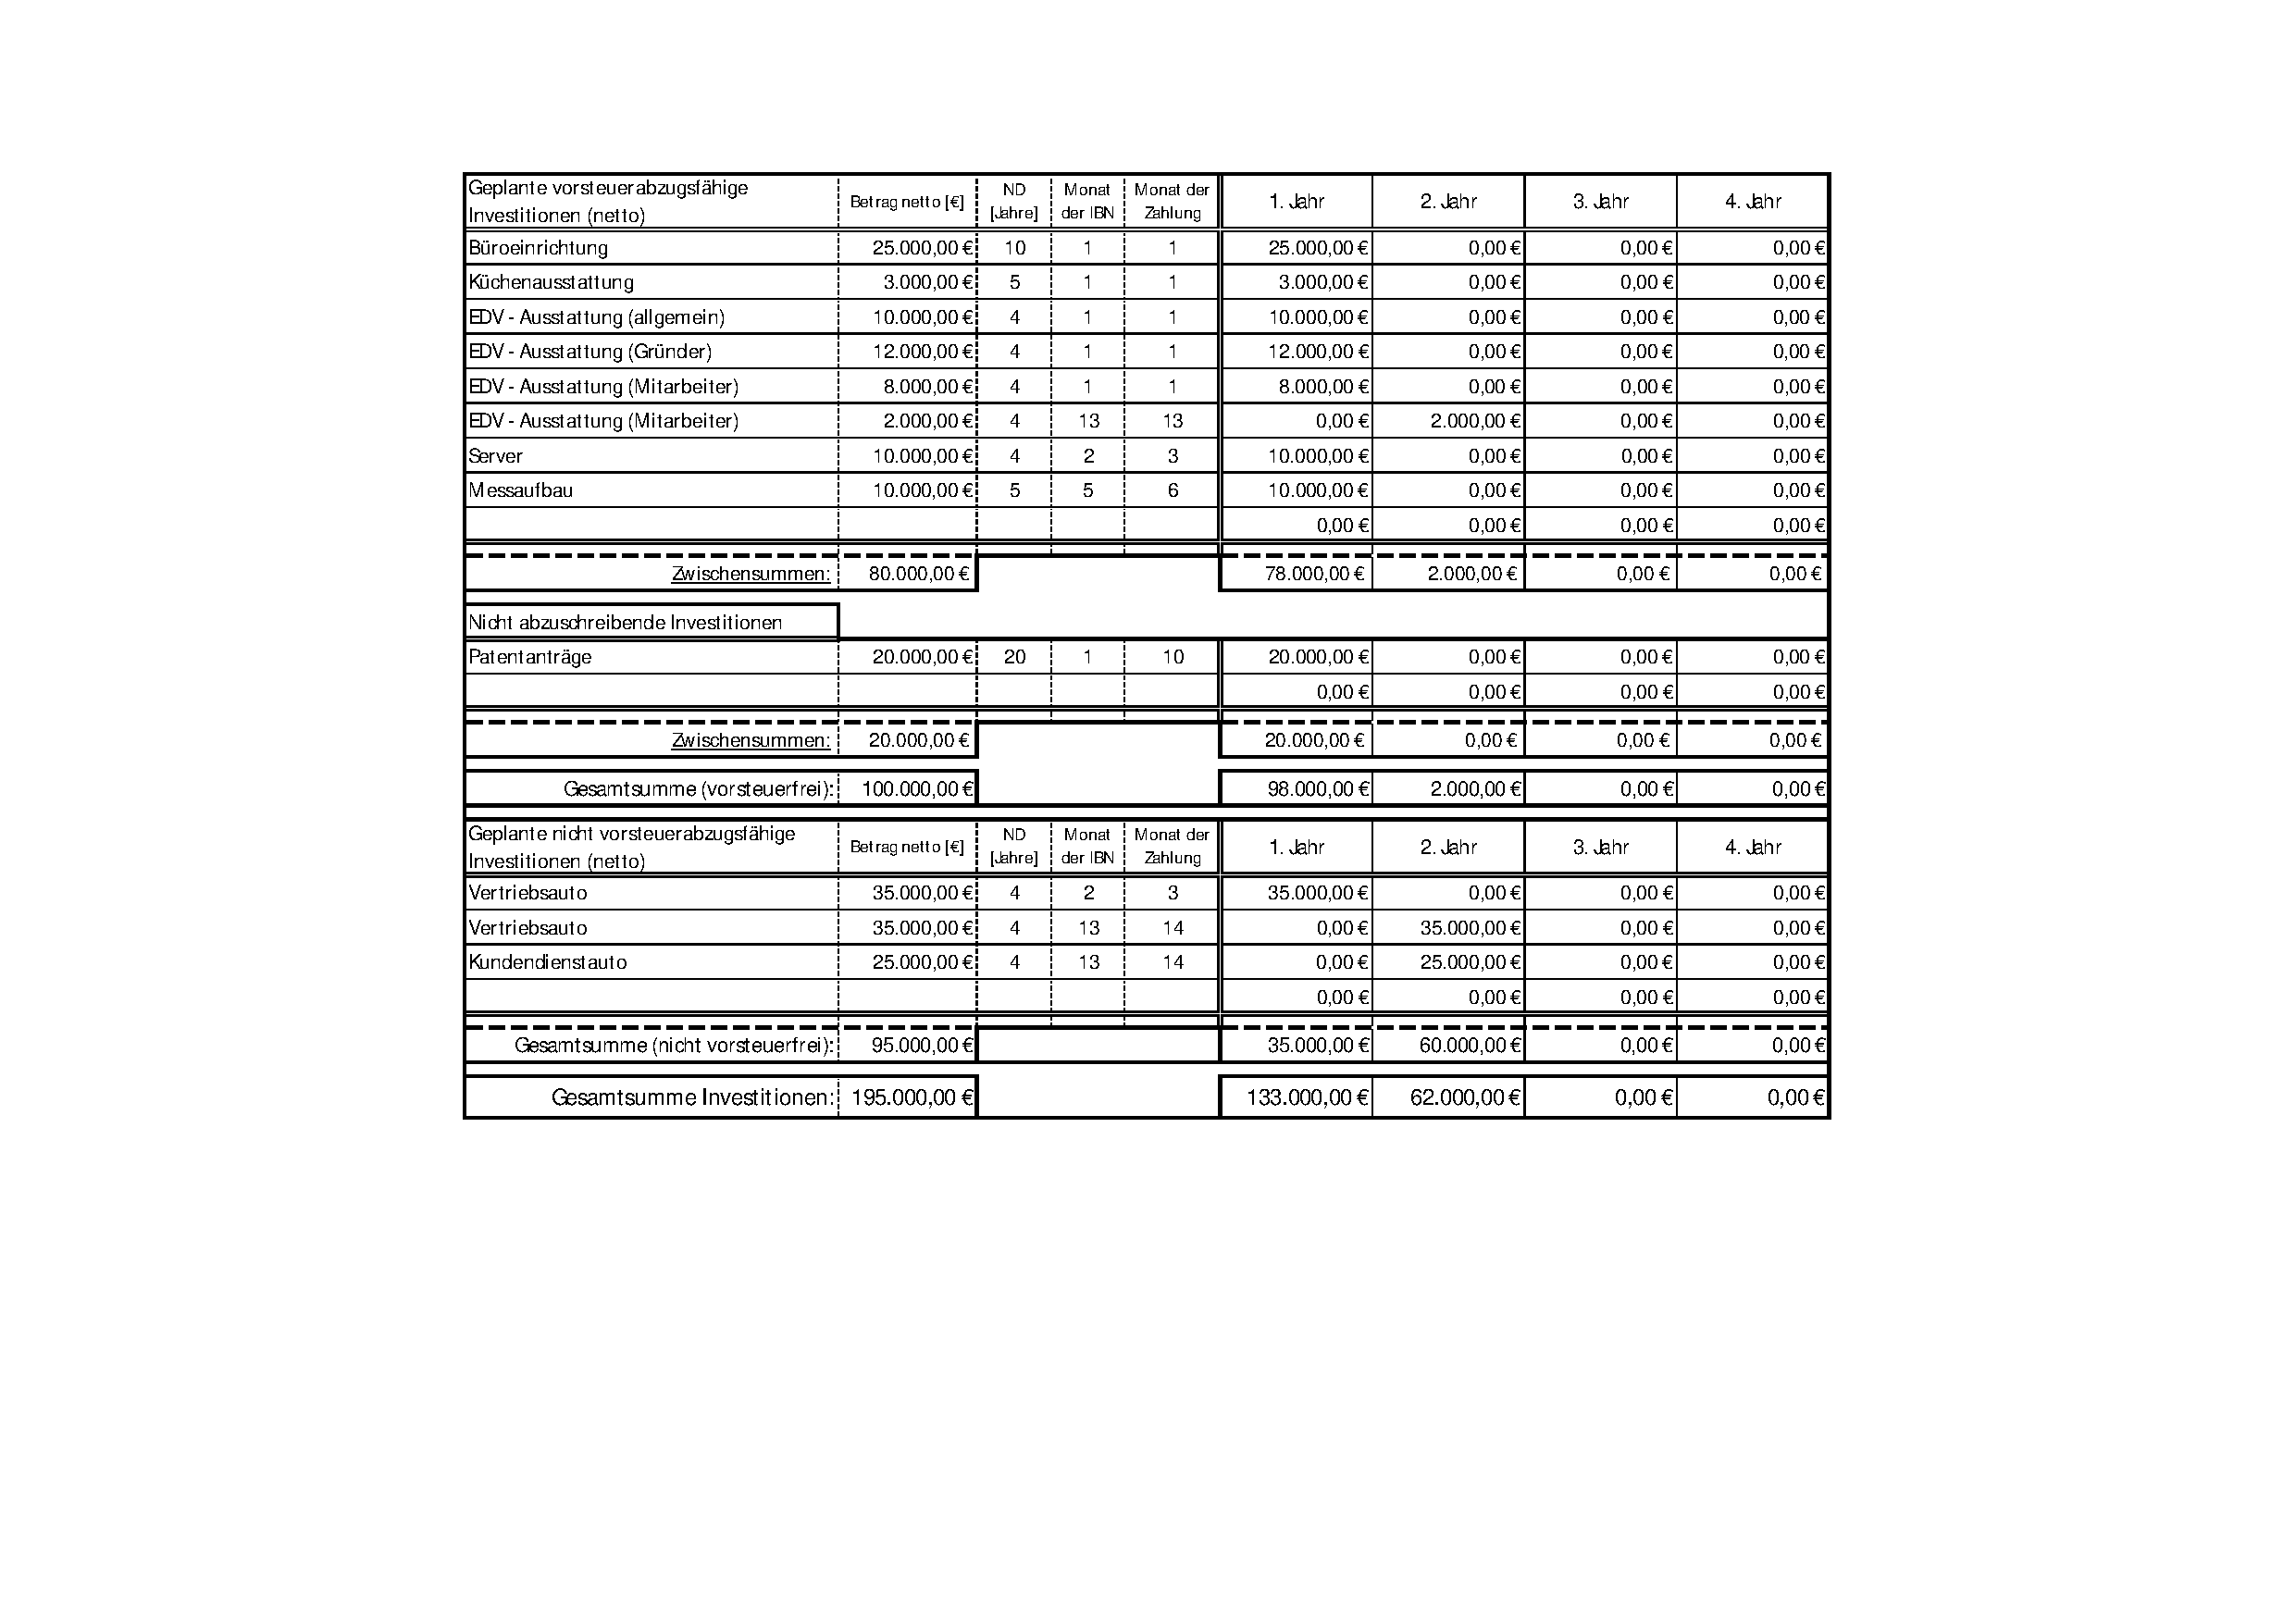
\includegraphics[width=15cm]{BasisSzenario-Investitionen.pdf}
	\caption{Investitionen im Basis-Szenario}
	\label{fig:BasisSzenario-Investitionen}
\end{figure}

\begin{landscape}
	\subsection{Aufwände}
	\begin{figure}[htp!]
		\centering
		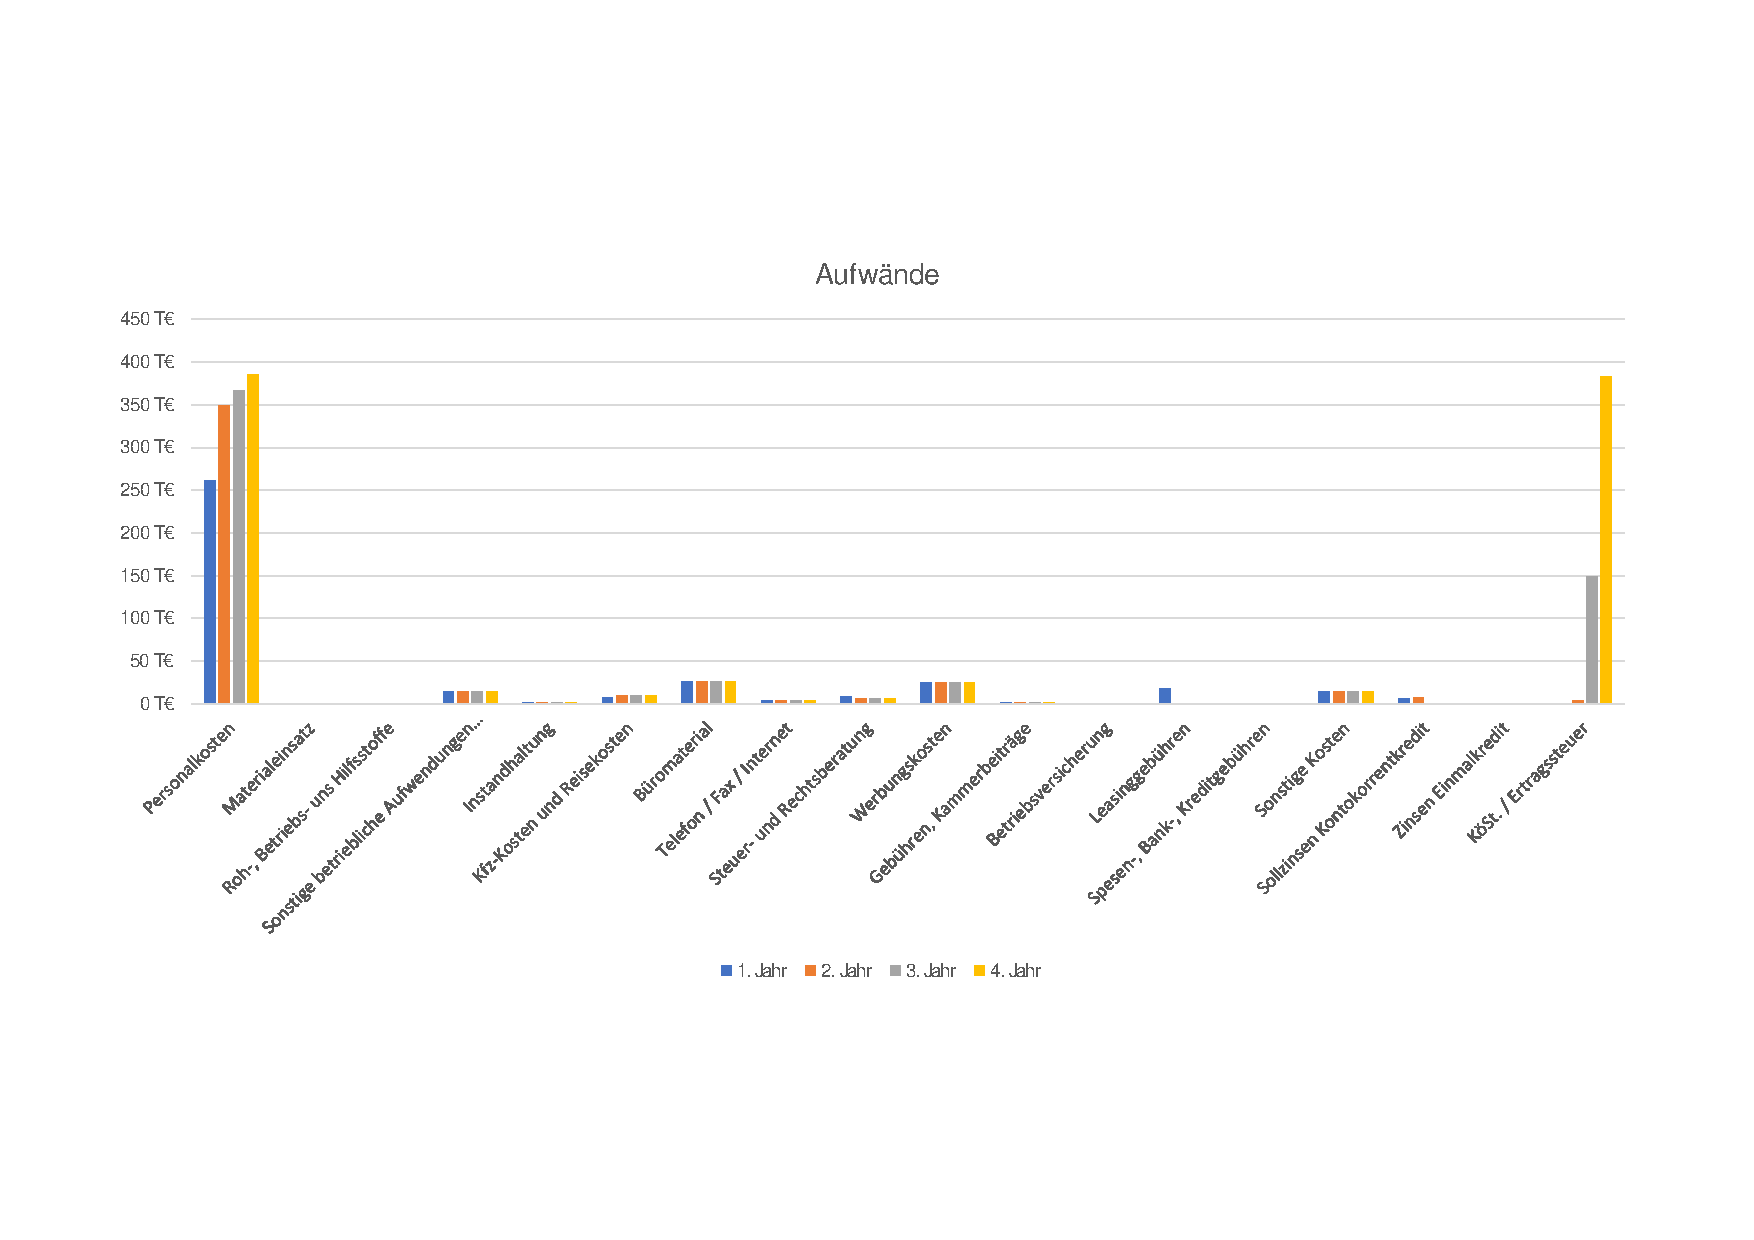
\includegraphics[width=24cm]{BasisSzenario-Aufwaende.pdf}
		\caption{Aufwände im Basis-Szenario}
		\label{fig:BasisSzenario-Aufwaende}
	\end{figure}
\end{landscape}

\newpage
\section{Best-Case-Szenario}
Für das Basis-Scenario wurden folgende Annahmen getroffen:
\begin{itemize}
	\item Es werden in den folgenden 4 Jahren 30 Neuentwicklungen in Auftrag gegeben (Aufteilung:~4/7/9/10). Damit werden $~17,6$\% der Robotertypen der 5 wichtigsten Hersteller mit dem System ausgerüstet, siehe Kapitel \ref{sec:Marketing}.
	\item Die Lizenzvergabe verteilt sich wie folgt:\newline (Angaben in Prozent vom weltweitem Absatz von Industrierobotern ($400.000$ Stück), siehe Kapitel \ref{sec:Marketing})
	\begin{itemize}
		\item 1. Jahr: $0,00$\% (0 Roboter)
		\item 2. Jahr: $0,05$\% (~200 Roboter)
		\item 3. Jahr: $0,20$\% (~800 Roboter)
		\item 4. Jahr: $1,00$\% (~4000 Roboter)
	\end{itemize}
	\item Die durchschnittliche Lizenzgebühr beträgt $1.500,00$\officialeuro.\\ Dies entspricht dem Mittelwert für $P_N = 1,50$kW -- $5,00$kW und $E_N = 10$\% -- $30$\%.
	\item Es wird mit 120 Teilnehmer an der Grundschulung innerhalb der nächsten 4 Jahren gerechnet (Aufteilung:~8/24/36/52). Zusätzlich nehmen 25 Teilnehmer die Intensivschulung in Anspruch (Aufteilung: 0/5/8/12).
\end{itemize}

\subsection{Break-Even-Point}
Der BEP wird im Best-Case-Szenario bereits im 2. Jahr erreicht, siehe Abbildung \ref{fig:BestSzenario-BEP}.
\begin{figure}[h]
	\centering
	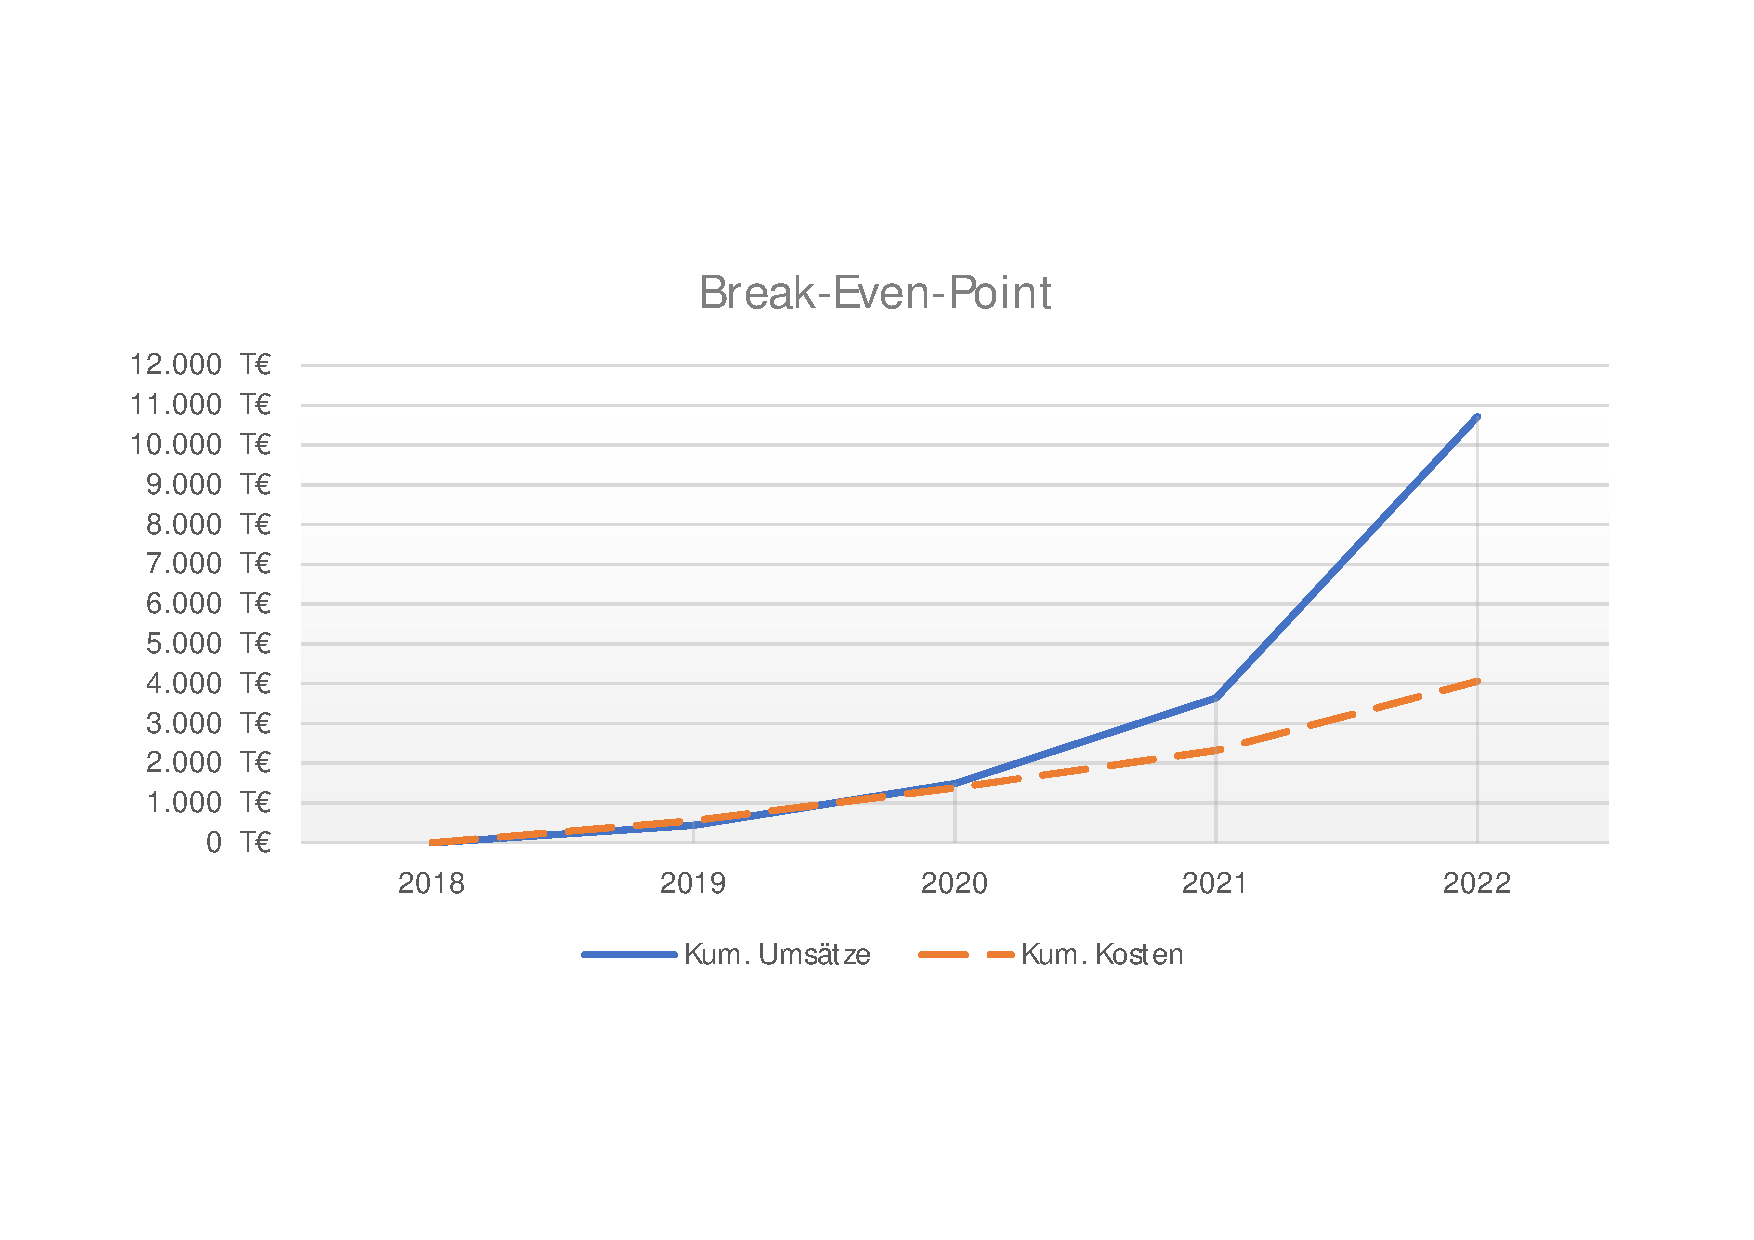
\includegraphics[width=15cm]{BestSzenario-BEP.pdf}
	\caption{Break-Even-Point im Best-Case-Szenario}
	\label{fig:BestSzenario-BEP}
\end{figure}

\subsection{Kapitalbedarf}
Der Kapitalbedarf bis zum BEP beträgt höchstens $120.000$\officialeuro.\\
Um diese Lücke zu schließen, werden folgende Finanzierungsmöglichkeiten geplant:
\begin{itemize}
	\item Einreichung eines Antrags bei der FFG im Basisprogramm zur Förderung von Einzelprojekten.
	\item UBG Gründerfonds
\end{itemize}
Dadurch ergibt sich folgende Finanzierung:\\
\begin{tabular}{l r}
	Kapitalbedarf & $-120.000$\officialeuro \\
	\hline
	FFG Basisprogramm(Projektsumme: $200.000$\officialeuro) & $+100.000$\officialeuro \\
	UBG Gründerfond & $+20.000$\officialeuro \\
	\bottomrule
\end{tabular}\\

\noindent Kurzfristige Liquiditätsschwankungen (spätere Zahlungen der Kunden, Projektvorfinanzierung, …) werden mit einem Kontokorrentkredit abgedeckt.

\newpage
\section{Worst-Case-Szenario}
Für das Basis-Scenario wurden folgende Annahmen getroffen:
\begin{itemize}
	\item Es werden in den folgenden 4 Jahren 10 Neuentwicklungen in Auftrag gegeben (Aufteilung:~1/2/3/4). Damit werden $~6$\% der Robotertypen der 5 wichtigsten Hersteller mit dem System ausgerüstet, siehe Kapitel \ref{sec:Marketing}.
	\item Die Lizenzvergabe verteilt sich wie folgt:\newline (Angaben in Prozent vom weltweitem Absatz von Industrierobotern ($400.000$ Stück), siehe Kapitel \ref{sec:Marketing})
	\begin{itemize}
		\item 1. Jahr: $0,00$\% (0 Roboter)
		\item 2. Jahr: $0,01$\% (~40 Roboter)
		\item 3. Jahr: $0,03$\% (~120 Roboter)
		\item 4. Jahr: $0,08$\% (~320 Roboter)
	\end{itemize}
	\item Die durchschnittliche Lizenzgebühr beträgt $1.500,00$\officialeuro.\\ Dies entspricht dem Mittelwert für $P_N = 1,50$kW -- $5,00$kW und $E_N = 10$\% -- $30$\%.
	\item Es wird mit 25 Teilnehmer an der Grundschulung innerhalb der nächsten 4 Jahren gerechnet (Aufteilung:~3/5/7/10). Zusätzlich nehmen 6 Teilnehmer die Intensivschulung in Anspruch (Aufteilung: 0/2/2/2).
\end{itemize}

\subsection{Break-Even-Point}
Der BEP wird im Worst-Case-Szenario erst im 4. Jahr erreicht, siehe Abbildung \ref{fig:WorstSzenario-BEP}.
\begin{figure}[h]
	\centering
	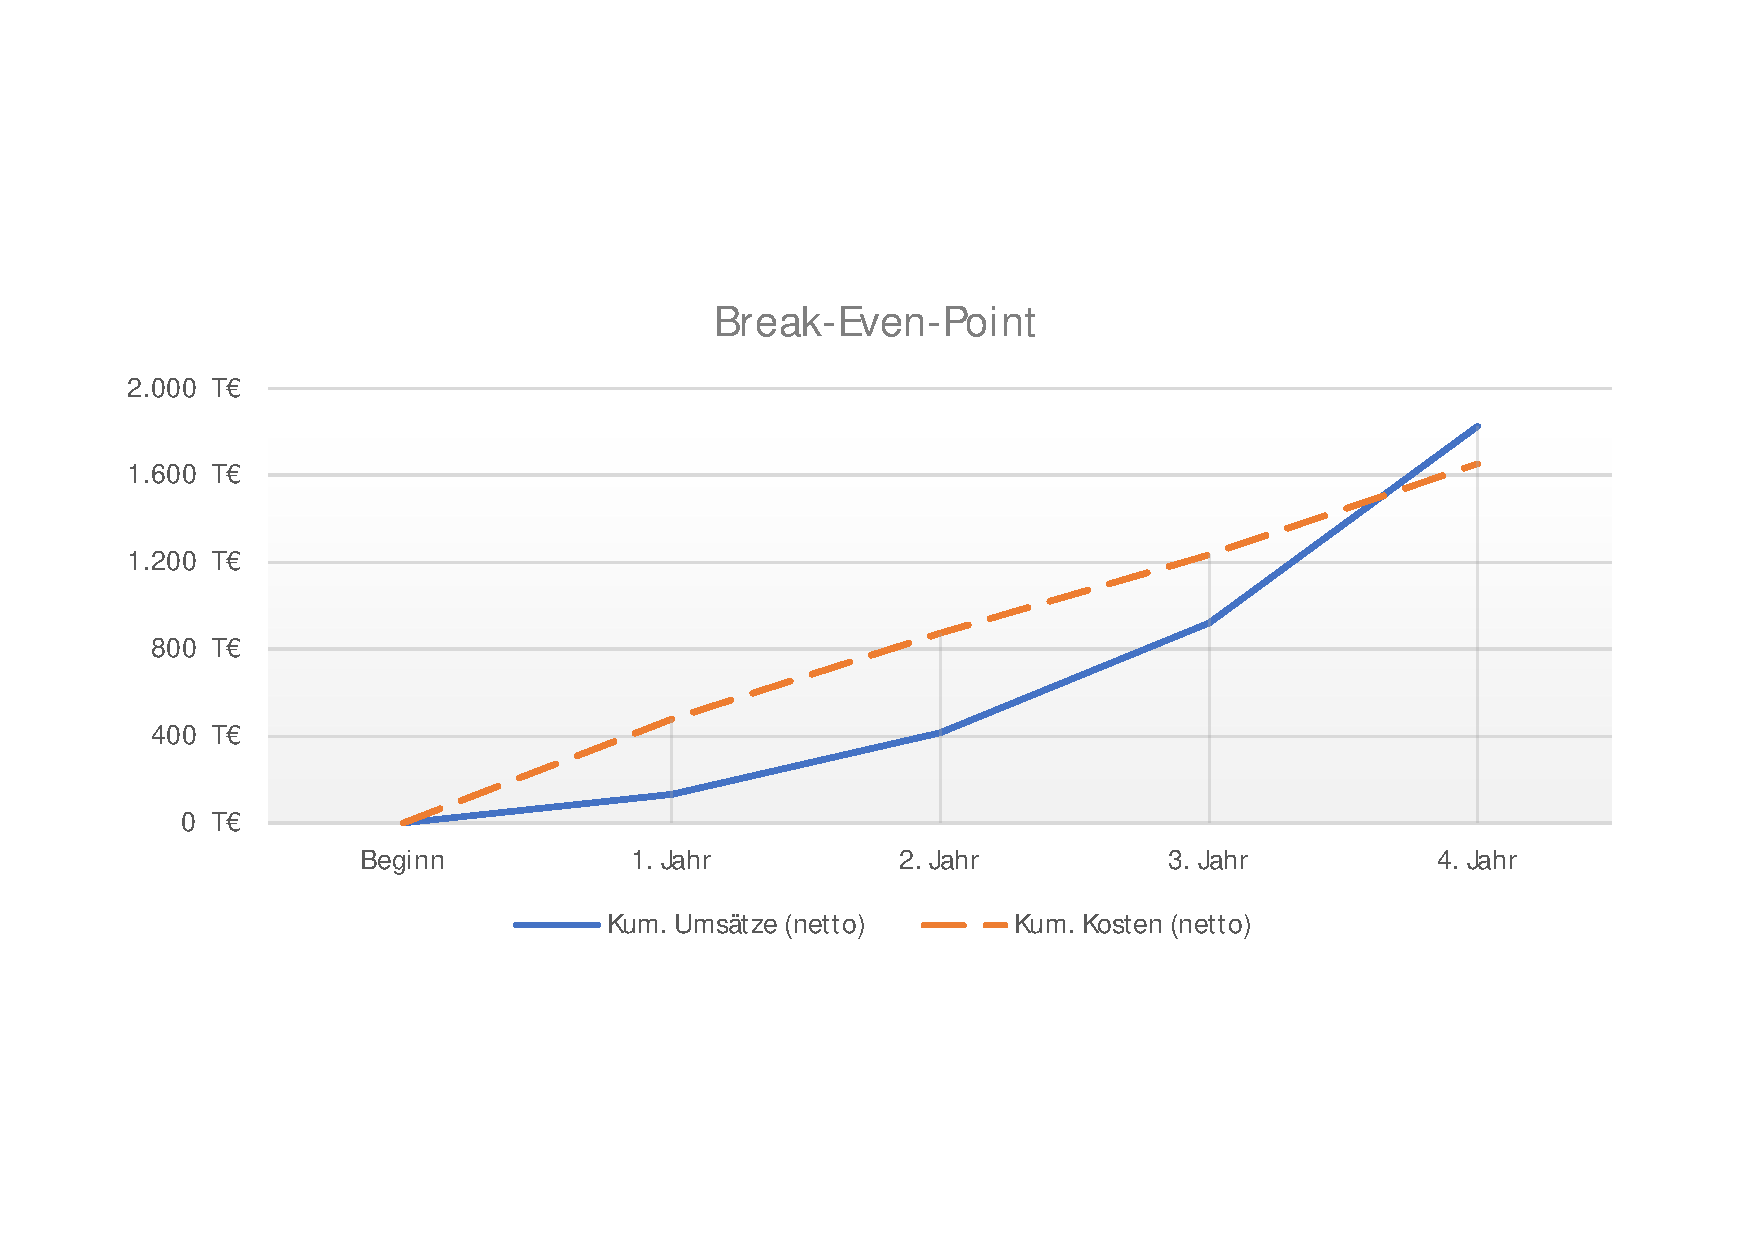
\includegraphics[width=15cm]{WorstSzenario-BEP.pdf}
	\caption{Break-Even-Point im Worst-Case-Szenario}
	\label{fig:WorstSzenario-BEP}
\end{figure}

\subsection{Kapitalbedarf}
Der Kapitalbedarf bis zum BEP beträgt höchstens $350.000$\officialeuro.\\
Um diese Lücke zu schließen, werden folgende Finanzierungsmöglichkeiten geplant:
\begin{itemize}
	\item Einreichung eines Antrags bei der FFG im Basisprogramm zur Förderung von Einzelprojekten.
	\item UBG Gründerfonds
\end{itemize}
Dadurch ergibt sich folgende Finanzierung:\\
\begin{tabular}{l r}
	Kapitalbedarf & $-350.000$\officialeuro \\
	\hline
	FFG Basisprogramm(Projektsumme: $200.000$\officialeuro) & $+100.000$\officialeuro \\
	UBG Gründerfond & $+75.000$\officialeuro \\
	\bottomrule
	Differenz: & $-175.000$\officialeuro
\end{tabular}\\

\textbf{Maßnahmen beim Eintritt des Worst-Case-Szenarios:}
\begin{itemize}
	\item Suche nach strategischen Investoren (Business Angels, Venture Capitalist, Roboterhersteller)
	\item Prüfung alternativer Förderungen
	\item Bankdarlehen im Zug der FFG-Förderung
\end{itemize}
Kurzfristige Liquiditätsschwankungen (spätere Zahlungen der Kunden, Projektvorfinanzierung, …) werden mit einem Kontokorrentkredit abgedeckt.